\section{Git Tags}
\begin{frame}[fragile]
  \slidetitle

  This section covers the following topics:
  \begin{itemize}
    \item Tag a git commit
    \item Checking out tags
  \end{itemize}
\end{frame}

\subsection{Make a tag}
\begin{frame}[fragile]
  \subslidetitle

  Select a short hash from the \cmd{git log --oneline} and let's make a tag:
  \begin{lstlisting}
(*\textcolor[HTML]{18B2B2}{(master)}*) $ (*\textcolor[HTML]{0000AA}{git tag v0.1 ed009a}*)
\end{lstlisting}
  \centerline{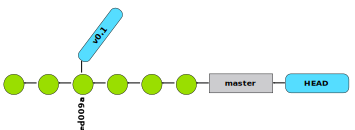
\includegraphics{assets/diagrams/git-tag.pdf}}

  \vspace{1em}
  Now we can checkout a tag using \cmd{git checkout}
  \begin{lstlisting}
(*\textcolor[HTML]{18B2B2}{(master)}*) $ (*\textcolor[HTML]{0000AA}{git checkout -b oldversion v0.1}*)
Switched to a new branch 'oldversion'
(*\textcolor[HTML]{18B2B2}{(oldversion)}*) $
\end{lstlisting}

\end{frame}

\subsection{Tag - Annotation}
\begin{frame}[fragile]
  \subslidetitle
  It is even possible to add heavier tags, called annotations. To do this use \cmd{git tag -a}.

  \begin{lstlisting}
(*\textcolor[HTML]{18B2B2}{(master)}*) $ (*\textcolor[HTML]{0000AA}{git tag -a v0.2 -m "example annotation tag"}*)
\end{lstlisting}

  Annotated tags add the following features:
  \begin{itemize}
    \item Tag message similar to commit message
    \item Name and email of the tagger
    \item Creation date
  \end{itemize}

  We can look at them using \cmd{git show}
  \begin{lstlisting}
(*\textcolor[HTML]{18B2B2}{(master)}*) $ (*\textcolor[HTML]{0000AA}{git show v0.2}*)
tag v0.2
Tagger: Tux Penguin <tux@penguin>
Date:   Tue Dec 1 03:17:04 2015 +0100

example annotation tag
...
\end{lstlisting}

\end{frame}

% git checkout branch which was edited a long time ago, and we can continue to edit at this stage.

\subsection{Summary}
\begin{frame}[fragile]
\subslidetitle
  What we've learned in this chapter:
  \begin{itemize}
    \item What a Tag is
    \item Ways to tag a commit
  \end{itemize}
\end{frame}
